\section{Auswertung}
\label{sec:Auswertung}

\subsection{Fouriesynthese}
Im ersten Teil des Experiments wurden wie in der Durchführung beschrieben die Spannungsverläufe zusammengesetzt. 

In Abbildung (\ref{fig:plot1}) ist die Fouriereihe der Sägezahnspannung zu sehen.
\begin{figure}[H]
  \centering
  \includegraphics[width = 0.6\linewidth]{Sägezahn.jpeg}
  \caption{Verlauf der Sägezahnspannung.}
  \label{fig:plot1}
\end{figure}

In Abbildung (\ref{fig:plot2}) ist die Fouriereihe der Dreiecksspannung zu erkennen. 
\begin{figure}[H]
  \centering
  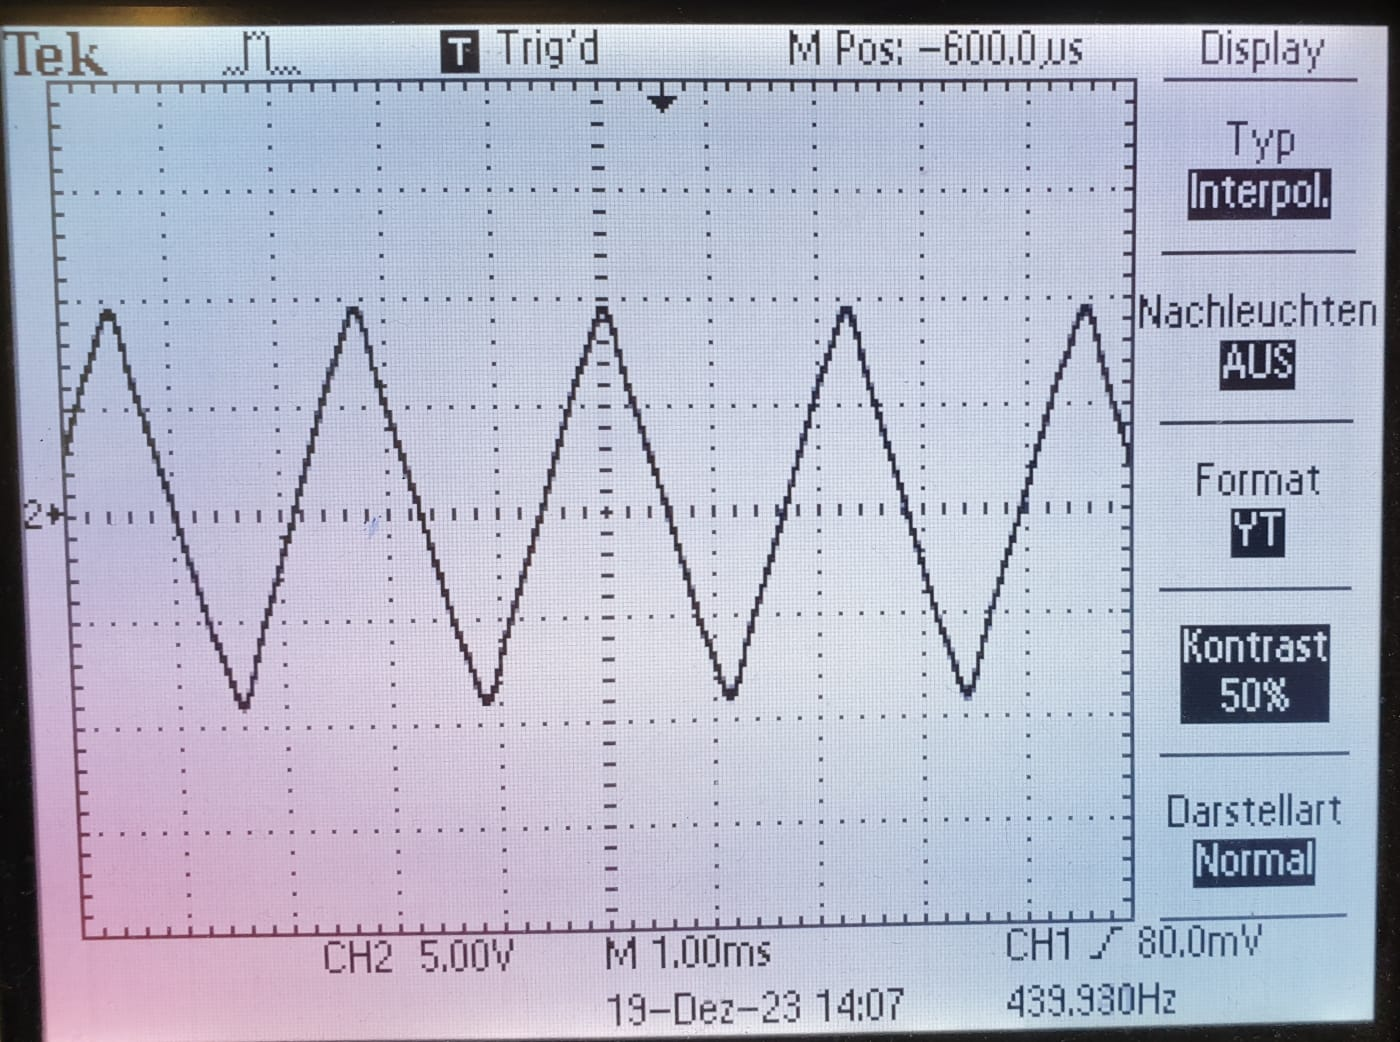
\includegraphics[width = 0.6\linewidth]{Dreieck.jpeg}
  \caption{Verlauf der Dreiecksspannung.}
  \label{fig:plot2}
\end{figure}

Außerdem ist in Abbildung (\ref{fig:plot3}) die Fouriereihe der Rechteckspannung zu sehen.
\begin{figure}[H]
  \centering
  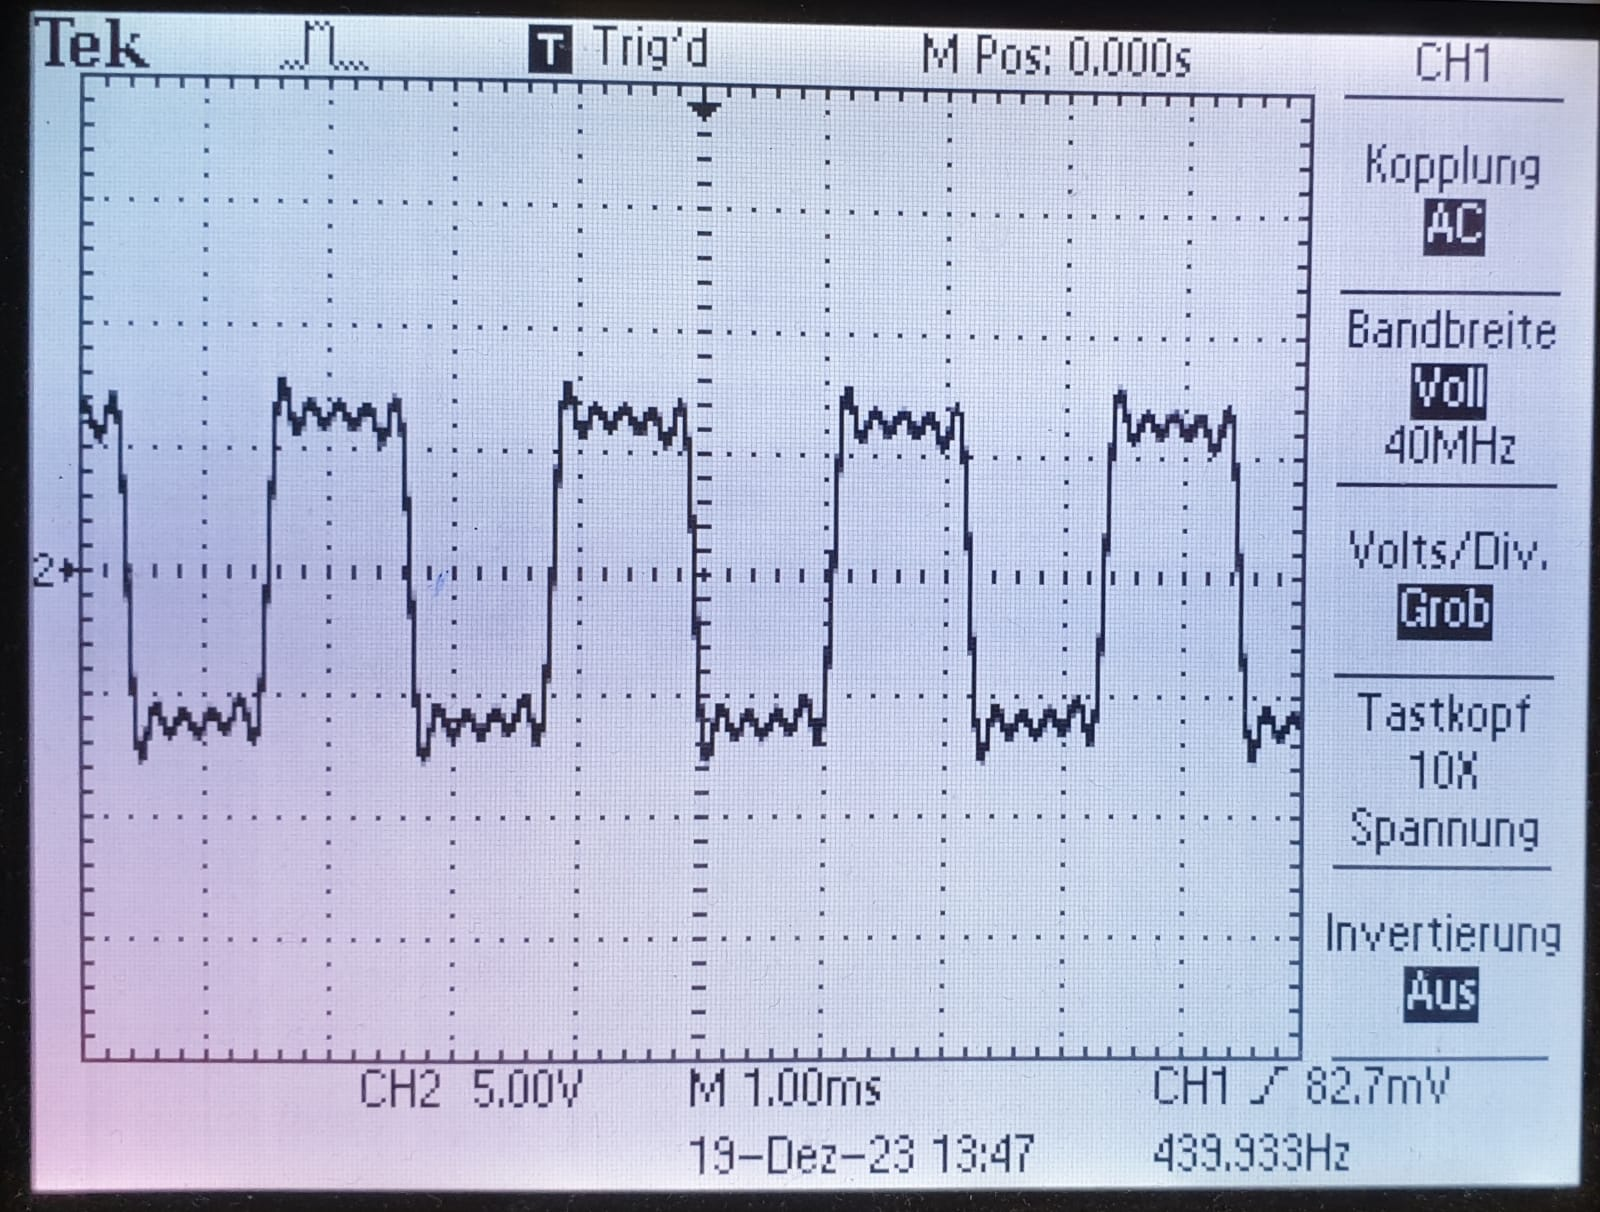
\includegraphics[width = 0.6\linewidth]{Viereck.jpeg}
  \caption{Verlauf der Rechteckspannung.}
  \label{fig:plot3}
\end{figure}

\subsection{Fourieanalyse}
Im zweiten Teil des Experiments wurde das Linienspektrums der Sägezahnspannung, Dreieckspannung und Rechteckspannung auf dem Oszilloskop eingestellt, um dann 
mithilfe des Cursers die Höhe der Peaks messen zu können. \\
\\
\textbf{Sägezahnspannung} \\
Die Frequenz wird in Kilohertz und die Höhe der Peaks wird in Dezibil gemessen. Die aufgenommenen Messdaten sind in Tabelle (\ref{tab:saegezahn}) aufgeführt. 
\begin{table}[H]
  \centering
  \caption{Gemessene Sägezahnspannung in Abhängigkeit der Frequenz.}
  \label{tab:saegezahn}
  \begin{tblr}{colspec={c c}}
      \toprule
      $f\,[\unit{\kilo\hertz}]$ & $U\,[\unit{\decibel}]$ \\
      \midrule
      10 & 33,0 \\
      20 & 27,0 \\
      30 & 23,4 \\
      40 & 21,0 \\
      50 & 19,0 \\
      60 & 17,4 \\
      70 & 16,2 \\
      80 & 14,6 \\
      90 & 13,4 \\
      100 & 13,0 \\
      110 & 12,2 \\
      \bottomrule
  \end{tblr}
\end{table}
Die Amplitude wird zur weiteren Betrachtung der Daten von Dezibil in Volt umgerechnet durch 
$$\unit{\volt} \sim  10 ^{\frac{\unit{\decibel}}{20}} \, .$$
Diese Messwerte werden in Abbildung (\ref{fig:saeg}) aufgetragen. Zusätzlich wird eine Ausgleichsfunktion berechnet, die durch
\begin{equation}
   U(x) = \symup{c} \cdot x^{\symup{d}} 
   \label{eqn:Ausgleichsfunktion}
\end{equation}
definiert ist. 
Für die Sägezahnspannung werden die Werte 
\begin{align*}
  \symup{c}_1 &= (451 \pm 4) \cdot 10^{-3} \, \unit{\volt\second} \\
  \symup{d}_1 &= -1,0036 \pm 0,0035
\end{align*}
berechnet. Diese Ausgleichsfunktion wird mit in Abbildung (\ref{fig:saeg}) abgebildet. 
\begin{figure}[H]
  \centering
  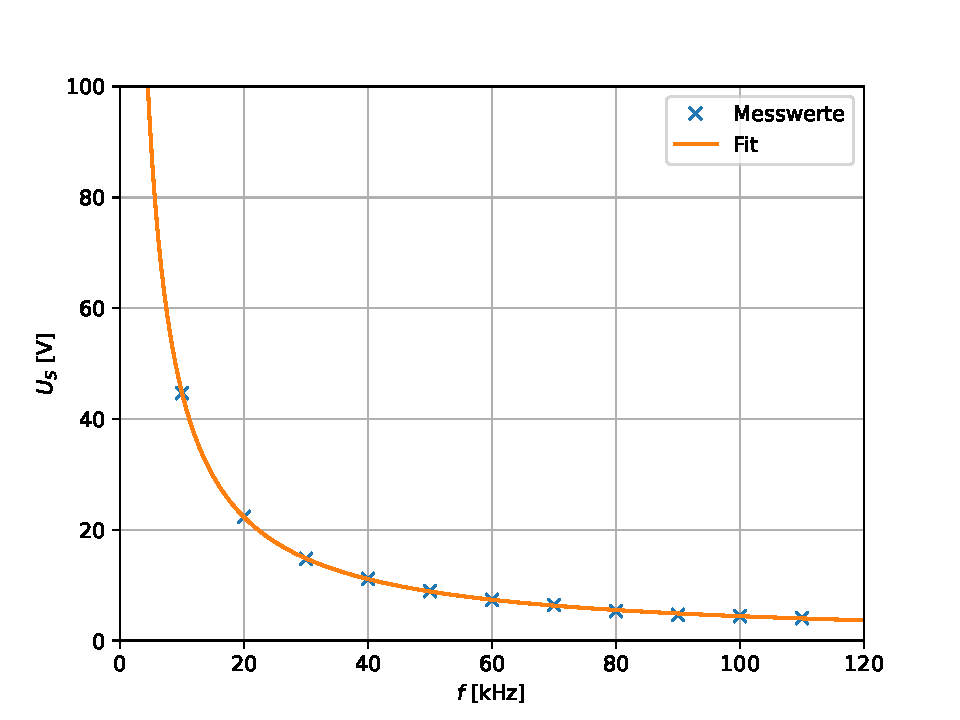
\includegraphics[width = 0.7\linewidth]{plot1.pdf}
  \caption{Gemessene Peaks der Sägezahnspannung $U_{\text{S}}$ und zugehörige Ausgleichsfunktion.}
  \label{fig:saeg}
\end{figure}
Der Faktor $\symup{d}$ zeigt welche Abhängigkeit der Höhe der Peaks von der Frequenz besteht. Das berechnete $\symup{d}_1 \approx -1$ bestätigt eine 
$\frac{1}{n}$ Abhängigkeit. \\
\\
\textbf{Dreiecksspannung} \\
Die gemessenen Peaks des Linienspektrums der Dreiecksspannung in Abhängigkeit von der Frequenz sind in Tabelle (\ref{tab:drei}) aufgeführt. 
\begin{table}[H]
  \centering
  \caption{Gemessene Dreieckspannung in Abhängigkeit der Frequenz.}
  \label{tab:drei}
  \begin{tblr}{colspec={c c}}
      \toprule
      $f\,[\unit{\kilo\hertz}]$ & $U\,[\unit{\decibel}]$ \\
      \midrule
      10 & 35,00 \\
      30 & 16,20 \\
      50 & 7,01 \\
      70 & 1,10 \\
      90 & -2,99 \\
      110 & -7,39 \\
      130 & -9,39 \\
      \bottomrule
  \end{tblr}
\end{table}
Durch diese Messwerte wird ebenfalls die Ausgleichsfunktion (\ref{eqn:Ausgleichsfunktion}) gelegt. Die durch diese Messwerte errechneten Faktoren sind 
\begin{align*}
  \symup{c}_2 &= (5381 \pm 91) \cdot 10^{-3} \, \unit{\volt\second} \\
  \symup{d}_2 &= -1,9809 \pm 0,0072 \, .
\end{align*}
Die Messwerte und die Ausgleichsfunktion sind in Abbildung (\ref{fig:drei}) dargestellt. 
\begin{figure}[H]
  \centering
  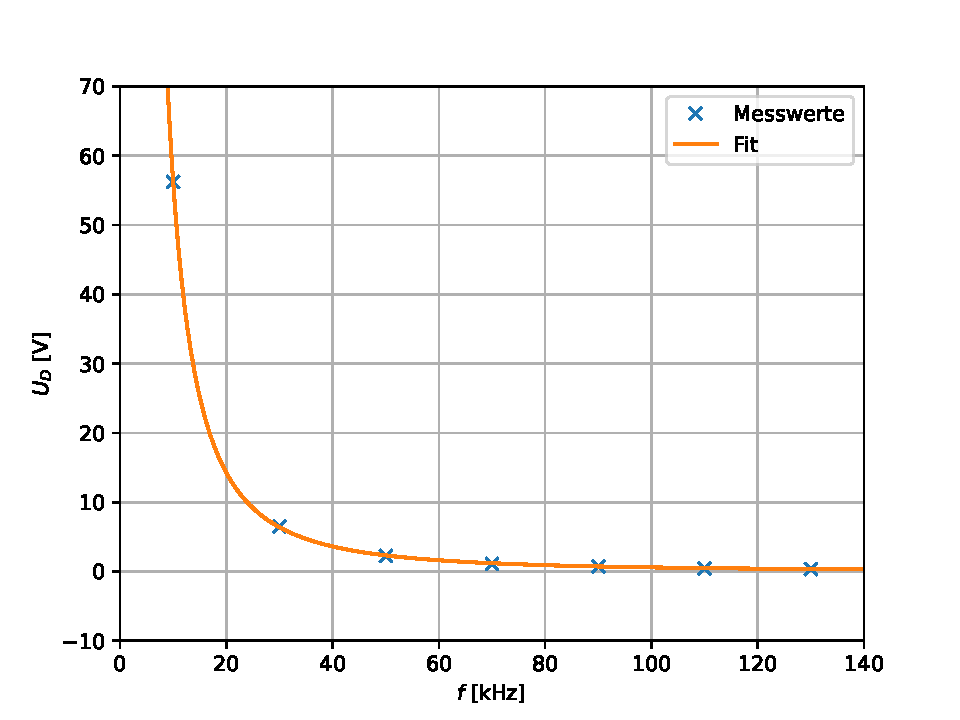
\includegraphics[width = 0.7\linewidth]{plot3.pdf}
  \caption{Gemessene Peaks der Dreieckspannung $U_{\text{D}}$ und Ausgleichsfunktion.}
  \label{fig:drei}
\end{figure}
Der Faktor $\symup{d}_2 \approx -2$ zeigt, dass die Höhe der Peaks mit $\frac{1}{n²}$ abfällt. \\
\\
\textbf{Rechteckspannung} \\
Die für die Peaks des Linienspektrums der Rechteckspannung aufgenommenen Messwerte sind in Tabelle (\ref{tab:recht}) notiert. 
\begin{table}[H]
  \centering
  \caption{Gemessene Rechteckspannung in Abhängigkeit der Frequenz.}
  \label{tab:recht}
  \begin{tblr}{colspec={c c}}
      \toprule
      $f\,[\unit{\kilo\hertz}]$ & $U\,[\unit{\decibel}]$ \\
      \midrule
      10 & 39,0 \\
      30 & 29,4 \\ 
      50 & 25,0 \\
      70 & 22,2 \\
      90 & 20,2 \\
      110 & 18,2 \\
      130 & 17,0 \\
      150 & 15,8 \\
      170 & 14,6 \\
      190 & 13,4 \\
      210 & 13,0 \\
      230 & 12,2 \\
      250 & 11,4 \\
      270 & 10,6 \\
      290 & 10,2 \\
      310 & 9,81 \\
      330 & 9,01 \\
      350 & 8,61 \\
      370 & 8,21 \\
      390 & 7,81 \\
      \bottomrule
  \end{tblr}
\end{table}
Die durch die Gleichung (\ref{eqn:Ausgleichsfunktion}) und die Messwerte aus Tabelle (\ref{tab:recht}) berechnete Ausgleichsgerade hat die Parameter
\begin{align*}
  \symup{c}_3 &= (878 \pm 5) \cdot 10^{-3} \, \unit{\volt\second} \\
  \symup{d}_3 &= -0,9939 \pm 0,0022 \, .
\end{align*}
Die Ausgleichsfunktion und Messwerte sind in Abbildung (\ref{fig:recht}) aufgetragen. 
\begin{figure}[H]
  \centering
  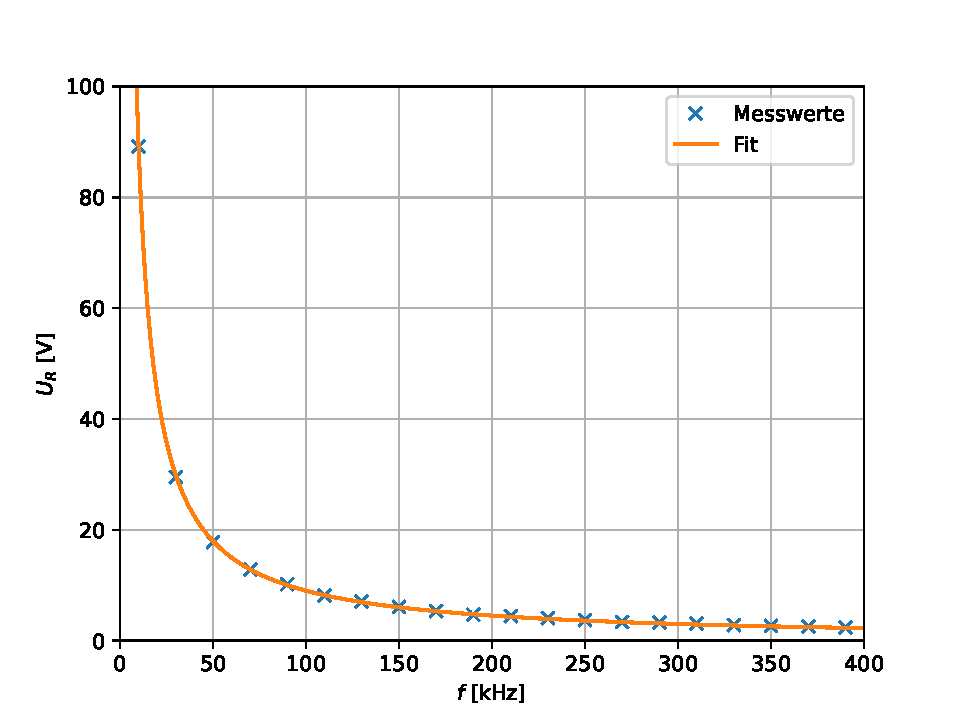
\includegraphics[width = 0.7\linewidth]{plot2.pdf}
  \caption{Gemessene Peaks der Rechteckspannung $U_{\text{R}}$ und Ausgleichsfunktion.}
  \label{fig:recht}
\end{figure}
Der Wert $\symup{d}_3 \approx -1$ weist auf eine $\frac{1}{n}$ Entwicklung der Höhe der Peaks des Linienspektrums hin. 


%a_saeg: 450.68807906140404, b_saeg: -1.0035509703352652
%a = 450.6881 ± 4.3789
%b = -1.0036 ± 0.0035
%a_recht: 877.8485996440896, b_recht: -0.993873520862041
%c = 877.8486 ± 5.1405
%d = -0.9939 ± 0.0022
%a_drei: 5381.273099208562, b_drei: -1.9808594085522564
%e = 5381.2731 ± 90.5629
%f = -1.9809 ± 0.0072


%Siehe \autoref{fig:plot}!